\documentclass[12pt,letterpaper]{article}
\usepackage[utf8]{inputenc}
\usepackage[left=2cm,right=2cm,top=2cm,bottom=2cm]{geometry}
\usepackage{multirow}
\title{Informe Oracle}
\author{Juan Rodriguez}
\date{November 2018}



\usepackage{graphicx}

\begin{document}
    
    \begin{center}
        
\includegraphics[width=4cm]{Imagenes/upt-logo.png}\\
        \vspace{12pt}
        \vspace{12pt}
        \large\textbf{UNIVERSIDAD PRIVADA DE TACNA}\\
        \vspace{12pt}
        \vspace{12pt}
        \large{FACULTAD DE INGENIERIA}\\
        \vspace{12pt}
        \vspace{12pt}
        \large{Escuela Profesional de Ingeniería de Sistemas}\\
        \vspace{12pt}
        \vspace{12pt}
        \textbf{INFORME LABORATORIO 5}\\
        \vspace{12pt}
        \vspace{12pt}
        Curso: Bases de Datos II\\
        \vspace{12pt}
        Docente: Ing. Patrick Cuadros\\
        \vspace*{12pt}
           \begin{flushleft}
        Alumno:\\
        \vspace{12pt}
        Rodriguez Mamani, Juan Rigoberto\hfill (2017057862)\\

        \end{flushleft}
        \vspace{100pt}

        Tacna – Perú\\
            2018
        \vspace{12pt}

            \thispagestyle{empty} % CARATULA SIN NUMERO
            \setcounter{page}{0} % REINICIAR CONTADOR DE PAGINAS
    \end{center}
    \break
    
\section{Cuestionario}
\vspace{12pt}
\begin{center}

\includegraphics[width=10cm]{Imagenes/Oracle_logo.png}\\
\end{center}
\vspace{12pt}
\subsection{¿Los valores introducidos al archivo sysctl.conf ¿Qué representan?}
\vspace{12pt}
{\hspace{12mm}Básicamente representan los valores de los parámetros del kernel, donde modificaremos la configuración de Oracle.} \\

\begin{center}
\textbf{Tabla de valores de los parámetros del kernel}
\end{center}
\begin{center}
  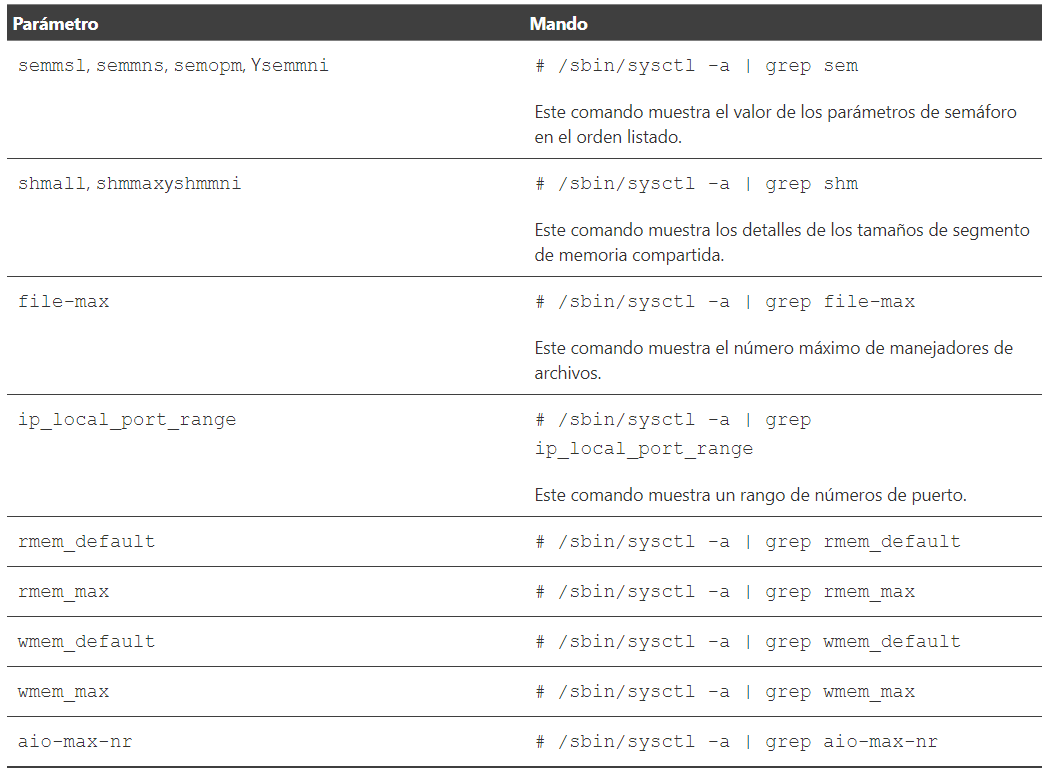
\includegraphics[width=14cm]{Imagenes/Tabla_parametros.png}\\
\end{center}


\subsection{¿Con qué usuario(s) puedo conectarme al servidor a través del Administrador Empresarial?}
\vspace{12pt}
{\hspace{12mm}Con el usuario: \textbf{SYS}} \\

\subsection{Capture una imagen de pantalla del navegador con el Administrador Empresarial, con el nombre de su servidor e iniciada la sesión del usuario SYS.}
\vspace{12pt}
\begin{center}
  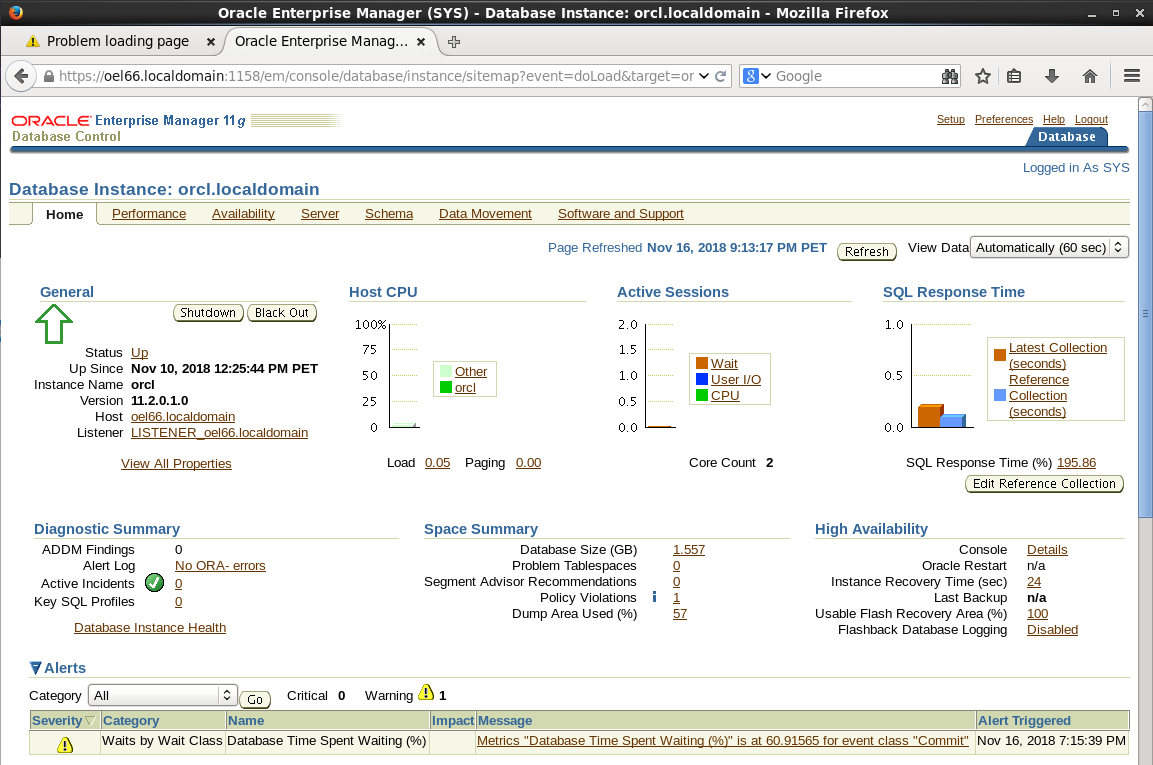
\includegraphics[width=16cm]{Imagenes/Oracle_servidor.png}\\
\end{center}
\break

\end{document}